\documentclass{ximera}
\usepackage{OERLinearAlgebra}


\usepackage{mathtools}
\usepackage{tikz-3dplot}
\newcommand\norm[1]{\left\lVert#1\right\rVert}

\author{Anna Davis \and Rosemarie Emanuele} \title{Dot Product and the Angle Between Vectors} \license{CC-BY 4.0}

\begin{document}

\begin{abstract}
 We state and prove the cosine formula for the dot product of two vectors, and show that two vectors are orthogonal if and only if their dot product is zero.
\end{abstract}
\maketitle


\section*{Angle Between Vectors} 
Given two vectors $\vec{u}$ and $\vec{v}$, let $\theta$ be the angle between them such that $0\leq\theta\leq \pi$.  We will refer to $\theta$ as the {\it included angle}.

\begin{image}[2in]
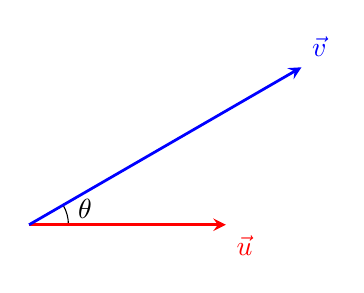
\begin{tikzpicture}
\draw (0.5,0)node[above=2mm, right=0mm]{$\theta$} arc (0:30:0.5) ;
\draw[line width=1pt,-stealth,red](0,0)--(2.5,0)node[below right]{$\vec{u}$};
\draw[line width=1pt,-stealth, blue](0,0)--(3.46,2)node[above right]{$\vec{v}$};
 \end{tikzpicture}
\end{image}

The following theorem establishes a relationship between the dot product and the included angle.

  \begin{theorem}\label{th:dotproductcosine} Let $\vec{u}$ and $\vec{v}$ be vectors in $\RR^n$, and let $\theta$ be the included angle.  Then
  \begin{equation*} \label{matlintrans}
 \vec{u}\cdot\vec{v}=\norm{\vec{u}}\norm{\vec{v}}\cos \theta
\end{equation*}
\end{theorem}


\begin{proof} Consider the triangle formed by $\vec{u}$, $\vec{v}$ and $\vec{u}-\vec{v}$. 

\begin{image}[2in]
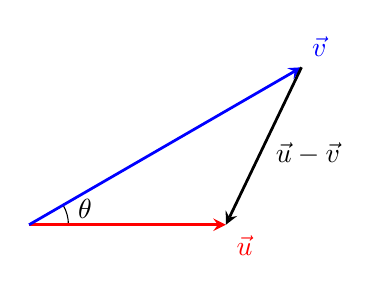
\begin{tikzpicture}
\draw (0.5,0)node[above=2mm, right=0mm]{$\theta$} arc (0:30:0.5) ;
\draw[line width=1pt,-stealth,red](0,0)--(2.5,0)node[below right]{$\vec{u}$};
\draw[line width=1pt,-stealth, blue](0,0)--(3.46,2)node[above right]{$\vec{v}$};
\draw[line width=1pt,-stealth](3.46,2)--(2.5,0)node[above=0.9cm, right=0.5cm]{$\vec{u}-\vec{v}$};
 \end{tikzpicture}
\end{image}

By the Law of Cosines we have:
\begin{align*}
\norm{\vec{u}-\vec{v}}^2=\norm{\vec{u}}^2+\norm{\vec{v}}^2-2\norm{\vec{u}}\norm{\vec{v}}\cos\theta
\end{align*}
By Theorem \ref{th:dotproductproperties}\ref{item:norm}
\begin{align*}
(\vec{u}-\vec{v})\cdot (\vec{u}-\vec{v})=&\vec{u}\cdot \vec{u}+\vec{v}\cdot \vec{v}-2\norm{\vec{u}}\norm{\vec{v}}\cos\theta
\end{align*}
By Theorem \ref{th:dotproductproperties}\ref{item:distributive-again}
\begin{align*}
(\vec{u}-\vec{v})\cdot \vec{u}-(\vec{u}-\vec{v})\cdot \vec{v}=&\vec{u}\cdot \vec{u}+\vec{v}\cdot \vec{v}-2\norm{\vec{u}}\norm{\vec{v}}\cos\theta
\end{align*}
By Theorem \ref{th:dotproductpropert ies}\ref{item:distributive}
\begin{align*}
\vec{u}\cdot \vec{u}-\vec{v}\cdot\vec{u}-\vec{u}\cdot\vec{v}+\vec{v}\cdot \vec{v}=&\vec{u}\cdot \vec{u}+\vec{v}\cdot \vec{v}-2\norm{\vec{u}}\norm{\vec{v}}\cos\theta
\end{align*}
By Theorem \ref{th:dotproductpropert ies}\ref{item:commutative}
\begin{align*}
-2(\vec{u}\cdot \vec{v})=&-2\norm{\vec{u}}\norm{\vec{v}}\cos\theta\\
\vec{u}\cdot \vec{v}=&\norm{\vec{u}}\norm{\vec{v}}\cos\theta
\end{align*}
\end{proof}

\begin{example}\label{ex:anglebetweenvectors}
Find the included angle between vectors $\vec{u}=\begin{bmatrix}2\\-1\\4\end{bmatrix}$ and $\vec{v}=\begin{bmatrix}1\\2\\-3\end{bmatrix}$.

\begin{explanation}
By Theorem \ref{th:dotproductcosine}, $\cos \theta=\frac{\vec{u}\cdot \vec{v}}{\norm{\vec{u}}\norm{\vec{v}}}$.  
$$\vec{u}\cdot\vec{v}=2-2-12=-12$$
$$\norm{\vec{u}}=\sqrt{4+1+16}=\sqrt{21}$$
$$\norm{\vec{v}}=\sqrt{1+4+9}=\sqrt{14}$$
$$\cos\theta =\frac{-12}{\sqrt{21}\sqrt{14}}$$
$$\theta \approx 134.4^{\circ}  $$
\end{explanation}
\end{example}

\section*{Orthogonal Vectors}

Two non-zero vectors are said to be \dfn{perpendicular} or \dfn{orthogonal} if the included angle is a right angle.


  \begin{theorem}\label{th:orth} Let $\vec{u}$ and $\vec{v}$ be non-zero vectors in $\RR^n$. Then $\vec{u}\cdot \vec{v}=0$ if and only if $\vec{u}$ and $\vec{v}$ are orthogonal.
\end{theorem}


\begin{proof} Recall that to prove an ``if and only if" statement, we must prove two statements.  In this particular case, we will need to show the following
\begin{itemize}
\item If $\vec{u}\cdot \vec{v}=0$, then $\vec{u}$ and $\vec{v}$ are orthogonal.
\item If $\vec{u}$ and $\vec{v}$ are orthogonal, then $\vec{u}\cdot \vec{v}=0$.
\end{itemize}
We leave the details of the proof to the reader.
\end{proof}

\section*{Practice Problems}
\begin{problem}
Find the degree measure of the included angle, $\theta$ for each pair of vectors.  Round your answers to the nearest tenth.
  \begin{problem}
  $\begin{bmatrix}1\\2\end{bmatrix}$ and $\begin{bmatrix}-3\\-1\end{bmatrix}$.
  
  Answer: $\theta=\answer{135}^\circ$
  \end{problem}
  
  \begin{problem}
  $\begin{bmatrix}-1\\2\\4\end{bmatrix}$ and $\begin{bmatrix}-2\\1\\-1\end{bmatrix}$
  
   Answer: $\theta=\answer{90}^\circ$
  \end{problem}

\begin{problem}
  $\begin{bmatrix}0\\-3\\1\end{bmatrix}$ and $\begin{bmatrix}-5\\-2\\4\end{bmatrix}$
  
   Answer: $\theta=\answer{61.9}^\circ$
  \end{problem}

\begin{problem}
  $\begin{bmatrix}1\\1\\-1\\2\end{bmatrix}$ and $\begin{bmatrix}-2\\0\\-3\\1\end{bmatrix}$
  
   Answer: $\theta=\answer{72.4}^\circ$
  \end{problem}
  
  \end{problem}

\begin{problem}
What does the sign of the dot product tell us about the included angle?
\end{problem}

\begin{problem}
Find all values of $a$ so that $\begin{bmatrix}a^2\\2a\\1\end{bmatrix}$ is orthogonal to $\begin{bmatrix}1\\2\\3\end{bmatrix}$.  List your answers in increasing order.

Answer: $\answer{-3}, \answer{-1}$.
\end{problem}

\begin{problem}
Find the value of $x$ for which the vector $\begin{bmatrix}x\\-4\end{bmatrix}$ is parallel to the vector $\begin{bmatrix}3\\2\end{bmatrix}$. What is the measure of the included angle, $\theta$? Find the measure of the included angle using Theorem \ref{ex:anglebetweenvectors}.  Do the two results agree?

Answer: 
$$x=\answer{-6}$$
$$\theta=\answer{180}^\circ$$
\end{problem}

\begin{problem}
Prove that if $\vec{u}$ is a unit vector, then $\vec{u}\cdot \vec{u}=1$.
\end{problem}

\begin{problem}
 Prove that if $\vec{u}_1$ and $\vec{u}_2$ are unit vectors, then $-1\leq\vec{u}_1\cdot \vec{u}_2\leq 1$.  In what cases are the extreme values of 1 and $-1$ attained?
\end{problem} 

\begin{problem}
 Imagine a clock with hands represented by vectors $\vec{m}$ and $\vec{h}$, as shown below.
At what whole hour will $\vec{m}\dotp\vec{h}$ attain its maximum value?  At what whole hour will $\vec{m}\dotp\vec{h}$ be as small as possible?

\begin{image}
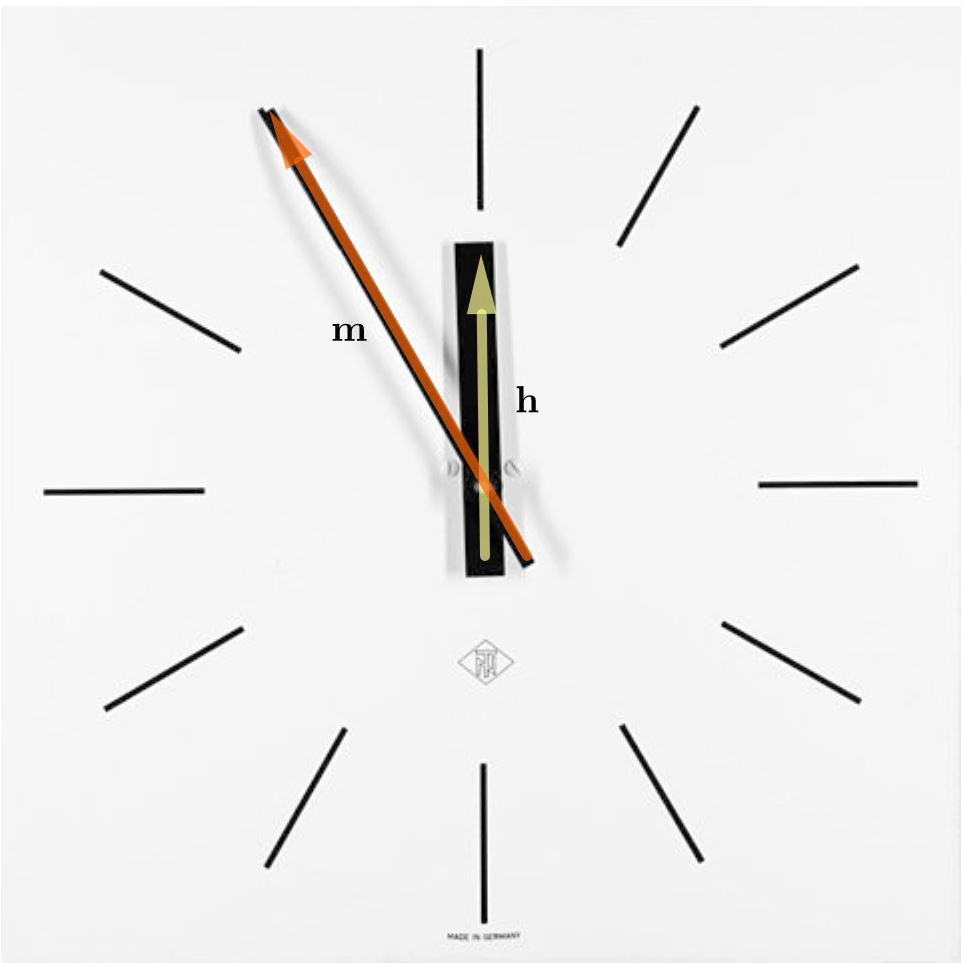
\includegraphics[height=3in]{clockvectors.jpg}
\end{image}

Answer:$$\vec{m}\dotp\vec{h}\text{ is greatest at }\answer{12}:00 \text{ o'clock}$$
$$\vec{m}\dotp\vec{h}\text{ is smallest at }\answer{6}:00 \text{ o'clock}$$
\end{problem}

\begin{problem} 
Let $O$ be a circle of radius $r$.  Suppose $A$ and $B$ are the endpoints of a diameter of $O$, and $C$ is a point on $O$ distinct from $A$ and $B$. Show that vectors $\overrightarrow{AC}$ and $\overrightarrow{BC}$ are orthogonal.  

\begin{hint}
Position the circle in the coordinate plane with center at the origin and segment $AB$ along the $x$-axis, as shown in the figure.
\end{hint}

\begin{image}[2.5in]
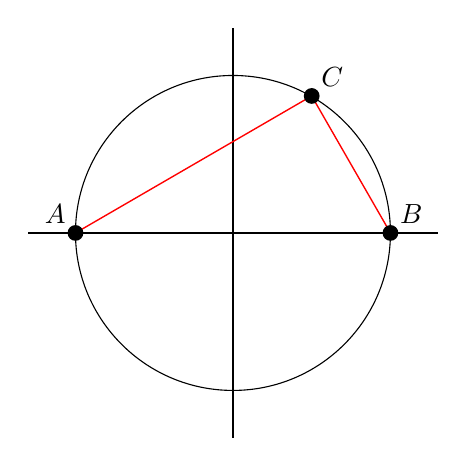
\begin{tikzpicture}[scale=2]

  \draw[] (-1.3,0)--(1.3,0);
  \draw[] (0,-1.3)--(0,1.3);
   
\draw[](0,0) circle (1cm);

    \draw[line width=0.5pt,red](-1,0)--(0.5,0.87);
   \draw[line width=0.5pt,red](1,0)--(0.5,0.87);
   
   \fill[] (1,0)node[above right]{$B$} circle (0.05cm);
   \fill[] (-1,0)node[above left]{$A$} circle (0.05cm);
   \fill[] (0.5,0.87)node[above right]{$C$} circle (0.05cm);
 \end{tikzpicture}
\end{image}
\end{problem}

\begin{problem} A rhombus is a quadrilateral with four congruent sides.  Use vectors to prove that a parallelogram is a rhombus if and only if its diagonals are perpendicular.
\begin{hint}
See the section on vector subtraction in Module VEC-M-0030.
\end{hint}
\end{problem}

%\section*{Photo Credits}
%The following images are courtesy of \href{https://commons.wikimedia.org/wiki/Main_Page}
%{Wikimedia Commons}

%\noindent Hannes Grobe (Figures \ref{fig:clock}), {\it Wall clock manufactured by Telefonbau \& Normalzeit.} CC-BY 3.0



\end{document} 